\documentclass[11pt]{article}
\usepackage[textwidth=18.0cm, textheight=23.0cm, top=2.0cm]{geometry}
\usepackage{pst-all}
\usepackage{amssymb}
\usepackage{tikz}
\usepackage{underscore}\begin{document}
\pagestyle{empty}


ClassName: \underline{\textbf{Class_08.2bp-18}}
\par
BinSize: \underline{\textbf{100 × 100}}
\par
ReduceSize: \underline{\textbf{100 × 100}}
\par
TypeNum: \underline{\textbf{39}}
\par
Num: \underline{\textbf{40}}
\par
OutS: \underline{\textbf{90000}}
\par
InS: \underline{\textbf{77075}}
\par
Rate: \underline{\textbf{0.856}}
\par
UB: \underline{\textbf{9}}
\par
LB0: \underline{\textbf{9}}
\par
LB: \underline{\textbf{9}}
\par
LBWithCut: \underline{\textbf{9}}
\par
NodeCut: \underline{\textbf{0}}
\par
ExtendedNodeCnt: \underline{\textbf{1}}
\par
GenNodeCnt: \underline{\textbf{1}}
\par
PrimalNode: \underline{\textbf{0}}
\par
ColumnCount: \underline{\textbf{9}}
\par
TotalCutCount: \underline{\textbf{0}}
\par
RootCutCount: \underline{\textbf{0}}
\par
LPSolverCnt: \underline{\textbf{1}}
\par
PricingSolverCnt: \underline{\textbf{0}}
\par
BranchAndBoundNum: \underline{\textbf{1}}
\par
isOpt: \underline{\textbf{true}}
\par
TimeOnInitSolution: \underline{\textbf{0.010 s}}
\par
TimeOnPrimal: \underline{\textbf{0.000 s}}
\par
TimeOnPricing: \underline{\textbf{0.000 s}}
\par
TimeOnRmp: \underline{\textbf{0.078 s}}
\par
TotalTime: \underline{\textbf{0.151 s}}
\par
\newpage


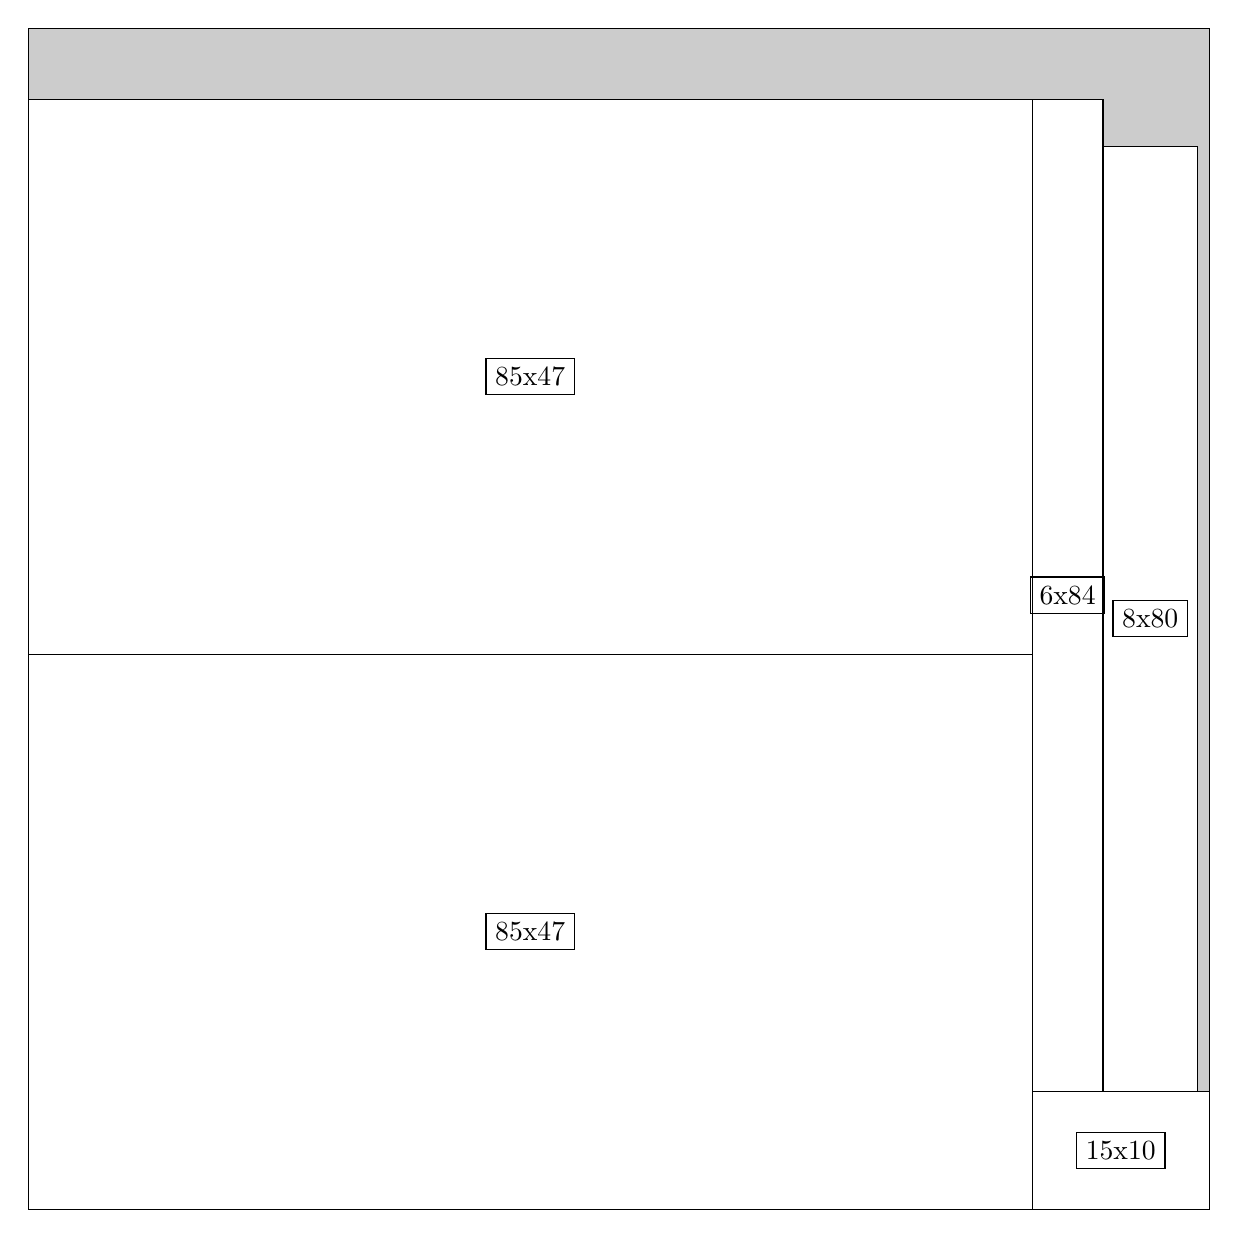
\begin{tikzpicture}[shorten >=1pt,scale=1.0,every node/.style={scale=1.0},->]
\tikzstyle{vertex}=[circle,fill=black!25,minimum size=14pt,inner sep=0pt]
\filldraw[fill=gray!40!white, draw=black] (0,0) rectangle (15.0,15.0);
\foreach \name/\x/\y/\w/\h in {85x47/0.0/0.0/12.75/7.05,85x47/0.0/7.05/12.75/7.05,8x80/13.65/1.5/1.2/12.0,6x84/12.75/1.5/0.8999999999999999/12.6,15x10/12.75/0.0/2.25/1.5}
\filldraw[fill=white!40!white, draw=black] (\x,\y) rectangle node[draw] (\name) {\name} ++(\w,\h);
\end{tikzpicture}


w =85 , h =47 , x =0 , y =0 , v =3995
\par
w =85 , h =47 , x =0 , y =47 , v =3995
\par
w =8 , h =80 , x =91 , y =10 , v =640
\par
w =6 , h =84 , x =85 , y =10 , v =504
\par
w =15 , h =10 , x =85 , y =0 , v =150
\par
\newpage


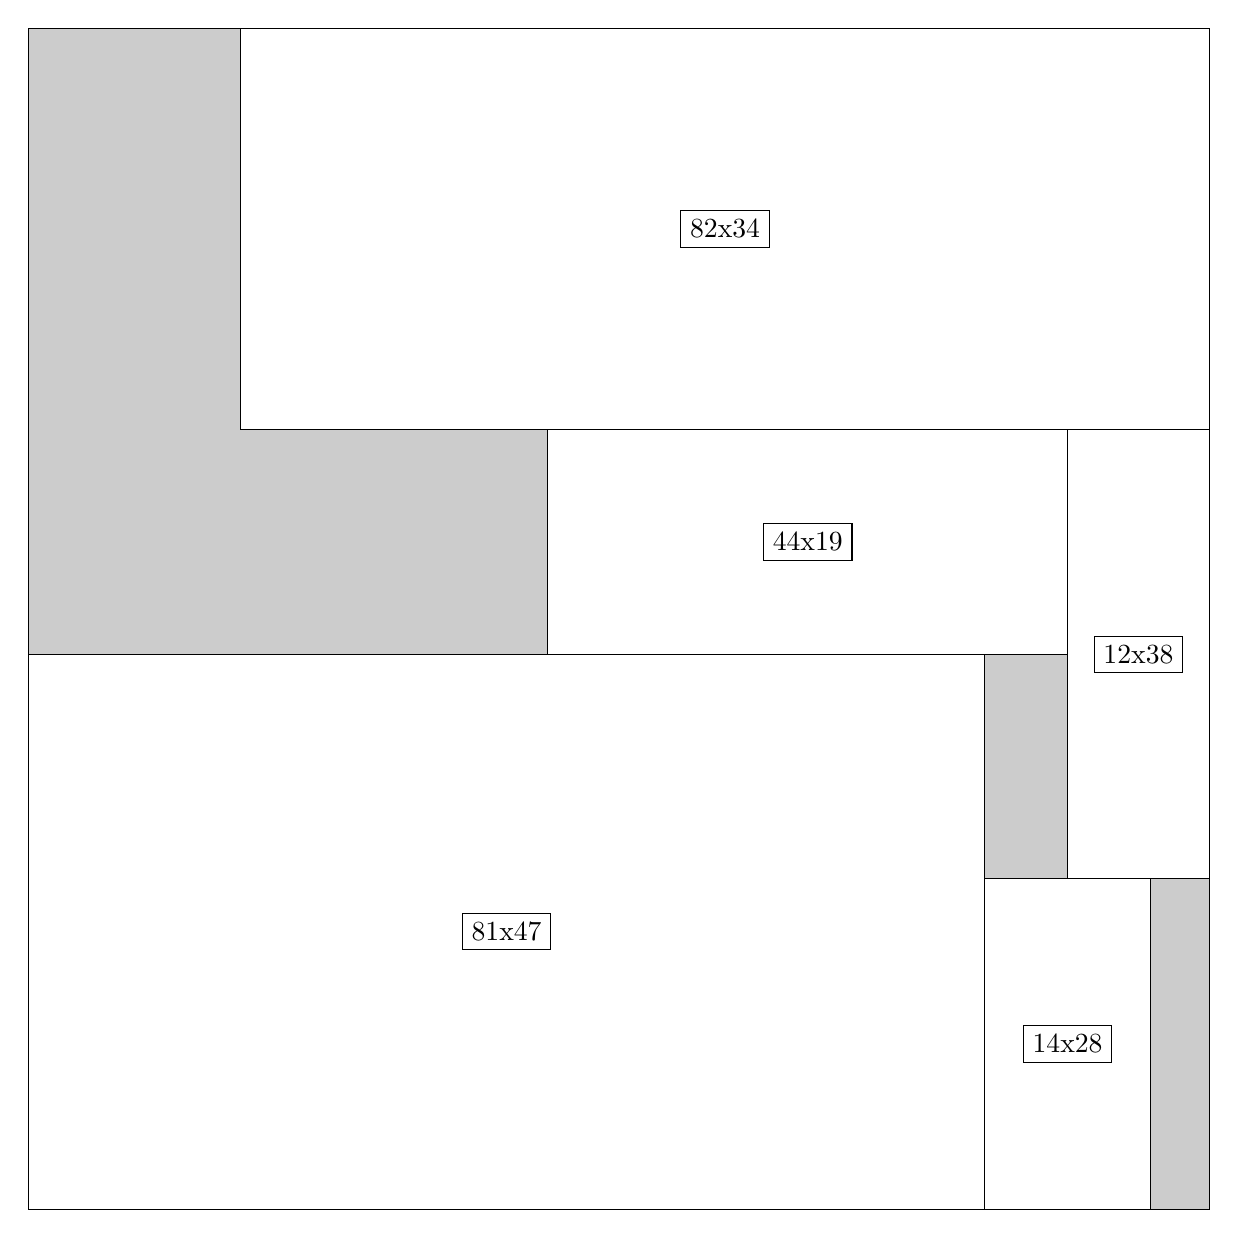
\begin{tikzpicture}[shorten >=1pt,scale=1.0,every node/.style={scale=1.0},->]
\tikzstyle{vertex}=[circle,fill=black!25,minimum size=14pt,inner sep=0pt]
\filldraw[fill=gray!40!white, draw=black] (0,0) rectangle (15.0,15.0);
\foreach \name/\x/\y/\w/\h in {81x47/0.0/0.0/12.15/7.05,82x34/2.6999999999999997/9.9/12.299999999999999/5.1,44x19/6.6/7.05/6.6/2.85,12x38/13.2/4.2/1.7999999999999998/5.7,14x28/12.15/0.0/2.1/4.2}
\filldraw[fill=white!40!white, draw=black] (\x,\y) rectangle node[draw] (\name) {\name} ++(\w,\h);
\end{tikzpicture}


w =81 , h =47 , x =0 , y =0 , v =3807
\par
w =82 , h =34 , x =18 , y =66 , v =2788
\par
w =44 , h =19 , x =44 , y =47 , v =836
\par
w =12 , h =38 , x =88 , y =28 , v =456
\par
w =14 , h =28 , x =81 , y =0 , v =392
\par
\newpage


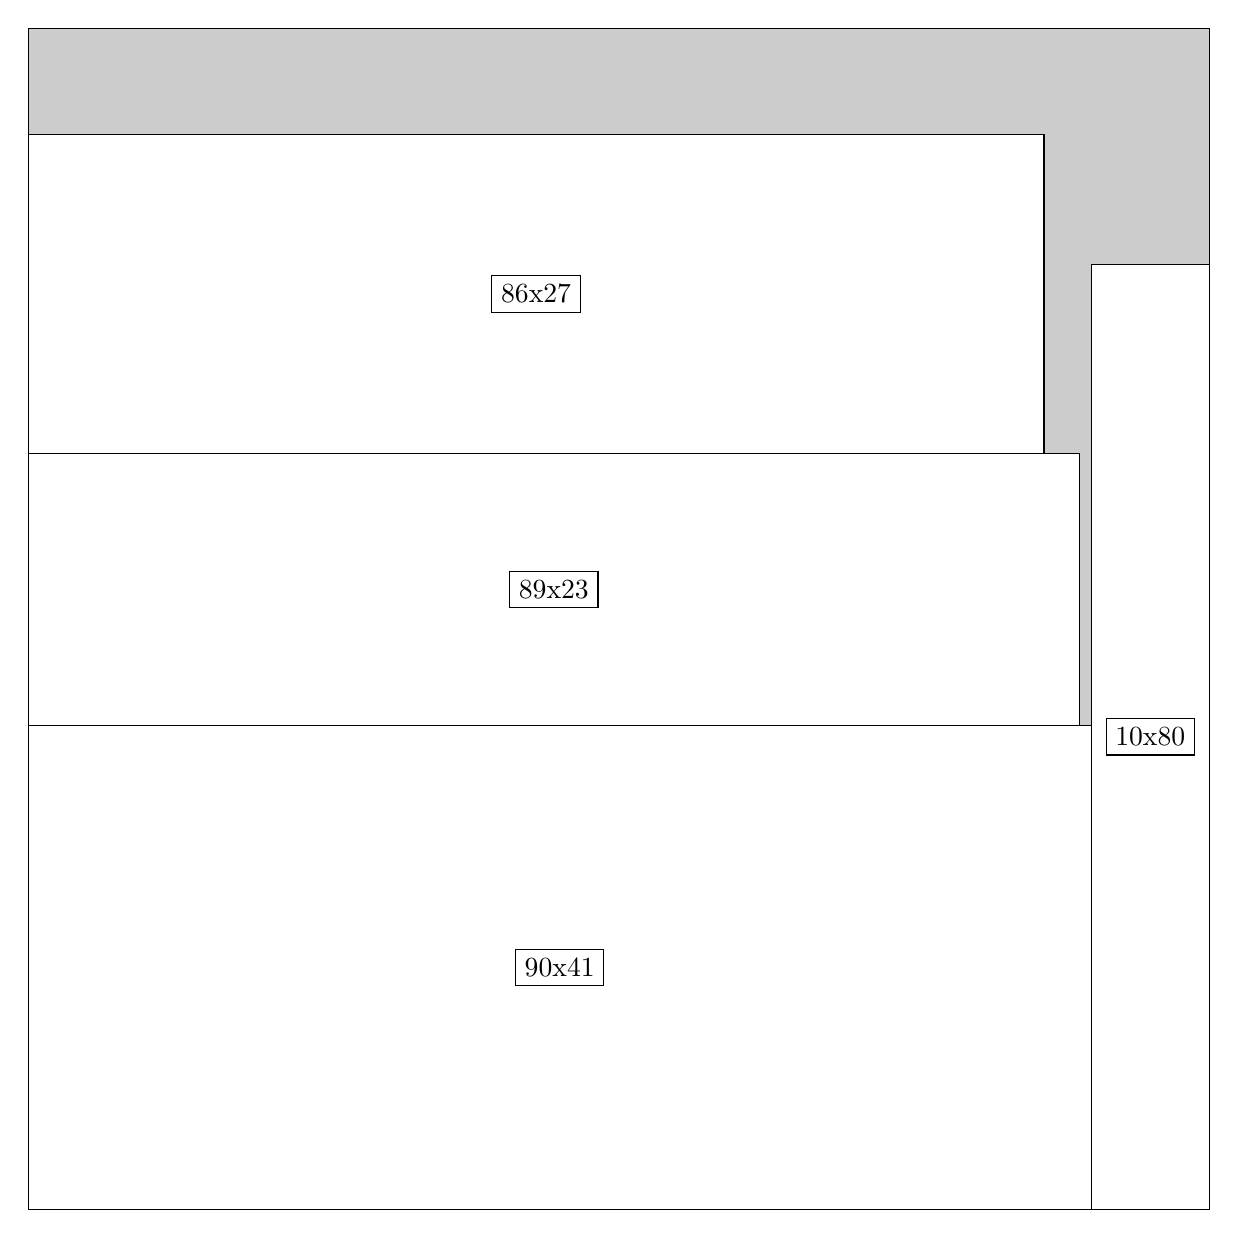
\begin{tikzpicture}[shorten >=1pt,scale=1.0,every node/.style={scale=1.0},->]
\tikzstyle{vertex}=[circle,fill=black!25,minimum size=14pt,inner sep=0pt]
\filldraw[fill=gray!40!white, draw=black] (0,0) rectangle (15.0,15.0);
\foreach \name/\x/\y/\w/\h in {90x41/0.0/0.0/13.5/6.1499999999999995,86x27/0.0/9.6/12.9/4.05,89x23/0.0/6.1499999999999995/13.35/3.4499999999999997,10x80/13.5/0.0/1.5/12.0}
\filldraw[fill=white!40!white, draw=black] (\x,\y) rectangle node[draw] (\name) {\name} ++(\w,\h);
\end{tikzpicture}


w =90 , h =41 , x =0 , y =0 , v =3690
\par
w =86 , h =27 , x =0 , y =64 , v =2322
\par
w =89 , h =23 , x =0 , y =41 , v =2047
\par
w =10 , h =80 , x =90 , y =0 , v =800
\par
\newpage


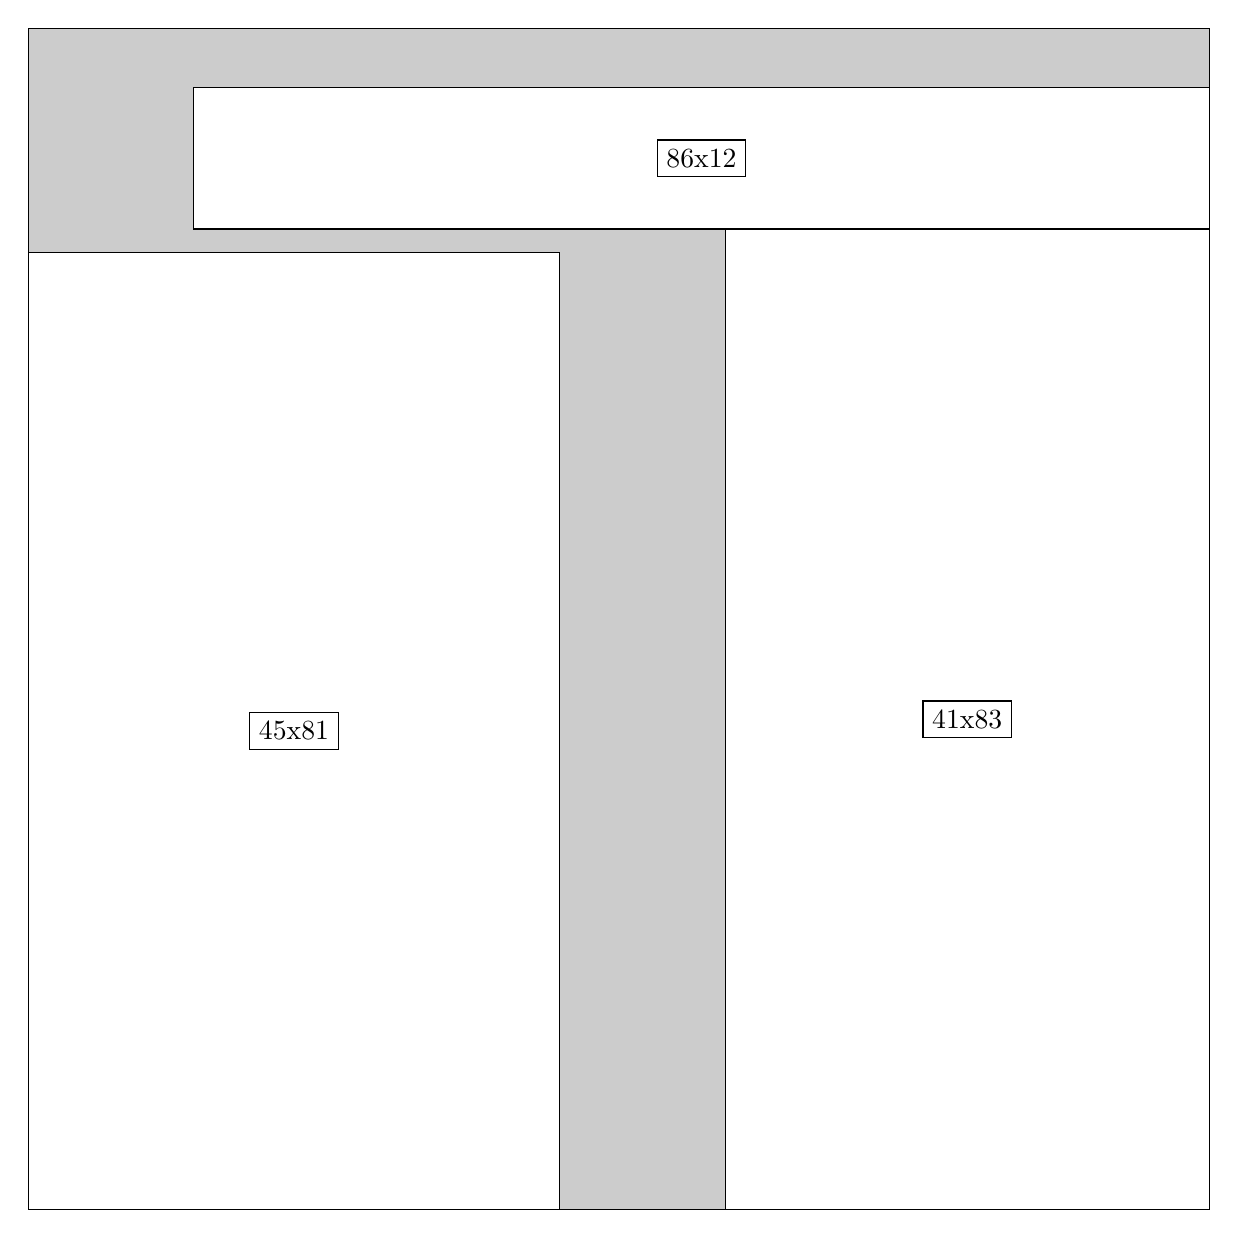
\begin{tikzpicture}[shorten >=1pt,scale=1.0,every node/.style={scale=1.0},->]
\tikzstyle{vertex}=[circle,fill=black!25,minimum size=14pt,inner sep=0pt]
\filldraw[fill=gray!40!white, draw=black] (0,0) rectangle (15.0,15.0);
\foreach \name/\x/\y/\w/\h in {45x81/0.0/0.0/6.75/12.15,41x83/8.85/0.0/6.1499999999999995/12.45,86x12/2.1/12.45/12.9/1.7999999999999998}
\filldraw[fill=white!40!white, draw=black] (\x,\y) rectangle node[draw] (\name) {\name} ++(\w,\h);
\end{tikzpicture}


w =45 , h =81 , x =0 , y =0 , v =3645
\par
w =41 , h =83 , x =59 , y =0 , v =3403
\par
w =86 , h =12 , x =14 , y =83 , v =1032
\par
\newpage


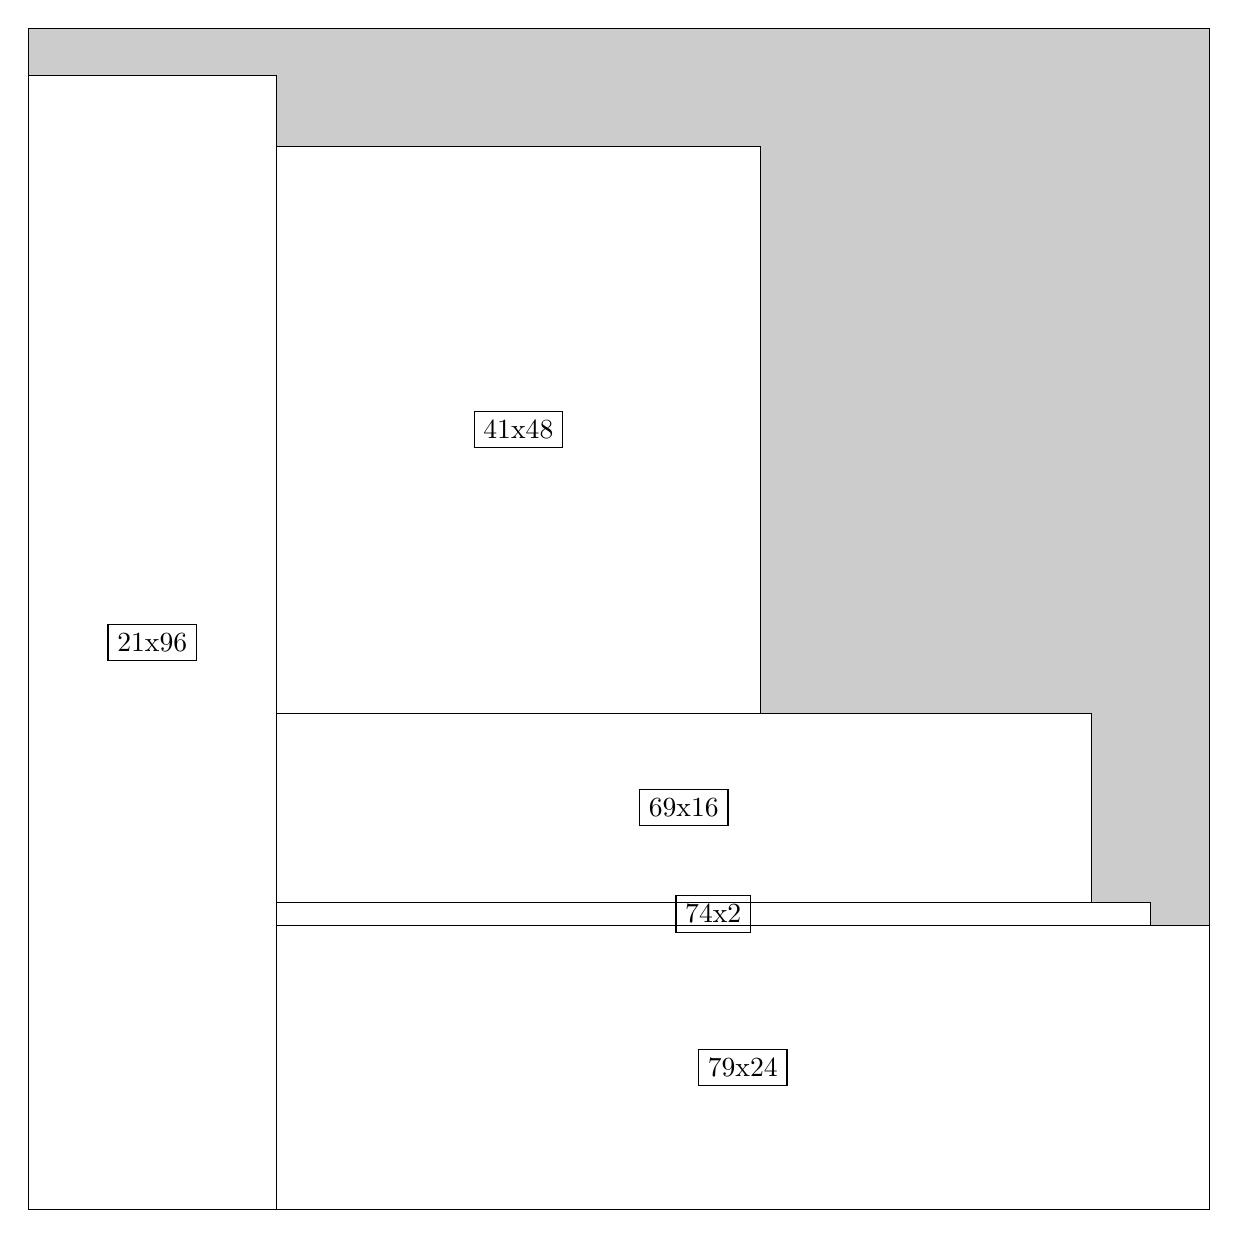
\begin{tikzpicture}[shorten >=1pt,scale=1.0,every node/.style={scale=1.0},->]
\tikzstyle{vertex}=[circle,fill=black!25,minimum size=14pt,inner sep=0pt]
\filldraw[fill=gray!40!white, draw=black] (0,0) rectangle (15.0,15.0);
\foreach \name/\x/\y/\w/\h in {21x96/0.0/0.0/3.15/14.399999999999999,79x24/3.15/0.0/11.85/3.5999999999999996,41x48/3.15/6.3/6.1499999999999995/7.199999999999999,69x16/3.15/3.9/10.35/2.4,74x2/3.15/3.5999999999999996/11.1/0.3}
\filldraw[fill=white!40!white, draw=black] (\x,\y) rectangle node[draw] (\name) {\name} ++(\w,\h);
\end{tikzpicture}


w =21 , h =96 , x =0 , y =0 , v =2016
\par
w =79 , h =24 , x =21 , y =0 , v =1896
\par
w =41 , h =48 , x =21 , y =42 , v =1968
\par
w =69 , h =16 , x =21 , y =26 , v =1104
\par
w =74 , h =2 , x =21 , y =24 , v =148
\par
\newpage


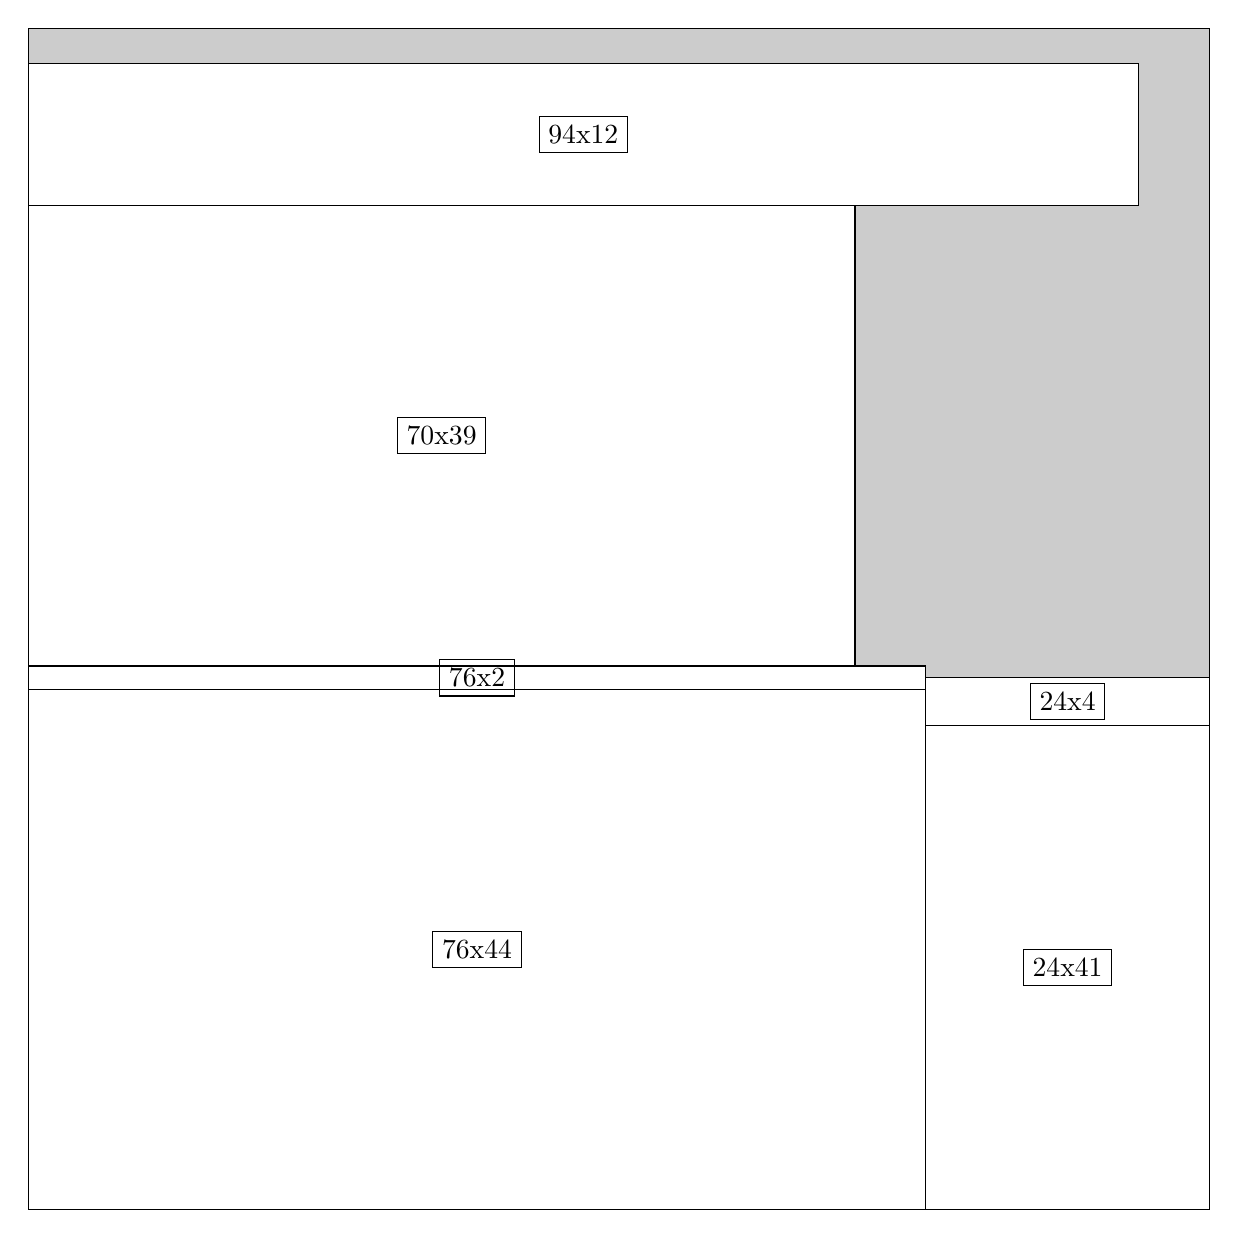
\begin{tikzpicture}[shorten >=1pt,scale=1.0,every node/.style={scale=1.0},->]
\tikzstyle{vertex}=[circle,fill=black!25,minimum size=14pt,inner sep=0pt]
\filldraw[fill=gray!40!white, draw=black] (0,0) rectangle (15.0,15.0);
\foreach \name/\x/\y/\w/\h in {76x44/0.0/0.0/11.4/6.6,70x39/0.0/6.8999999999999995/10.5/5.85,94x12/0.0/12.75/14.1/1.7999999999999998,24x41/11.4/0.0/3.5999999999999996/6.1499999999999995,76x2/0.0/6.6/11.4/0.3,24x4/11.4/6.1499999999999995/3.5999999999999996/0.6}
\filldraw[fill=white!40!white, draw=black] (\x,\y) rectangle node[draw] (\name) {\name} ++(\w,\h);
\end{tikzpicture}


w =76 , h =44 , x =0 , y =0 , v =3344
\par
w =70 , h =39 , x =0 , y =46 , v =2730
\par
w =94 , h =12 , x =0 , y =85 , v =1128
\par
w =24 , h =41 , x =76 , y =0 , v =984
\par
w =76 , h =2 , x =0 , y =44 , v =152
\par
w =24 , h =4 , x =76 , y =41 , v =96
\par
\newpage


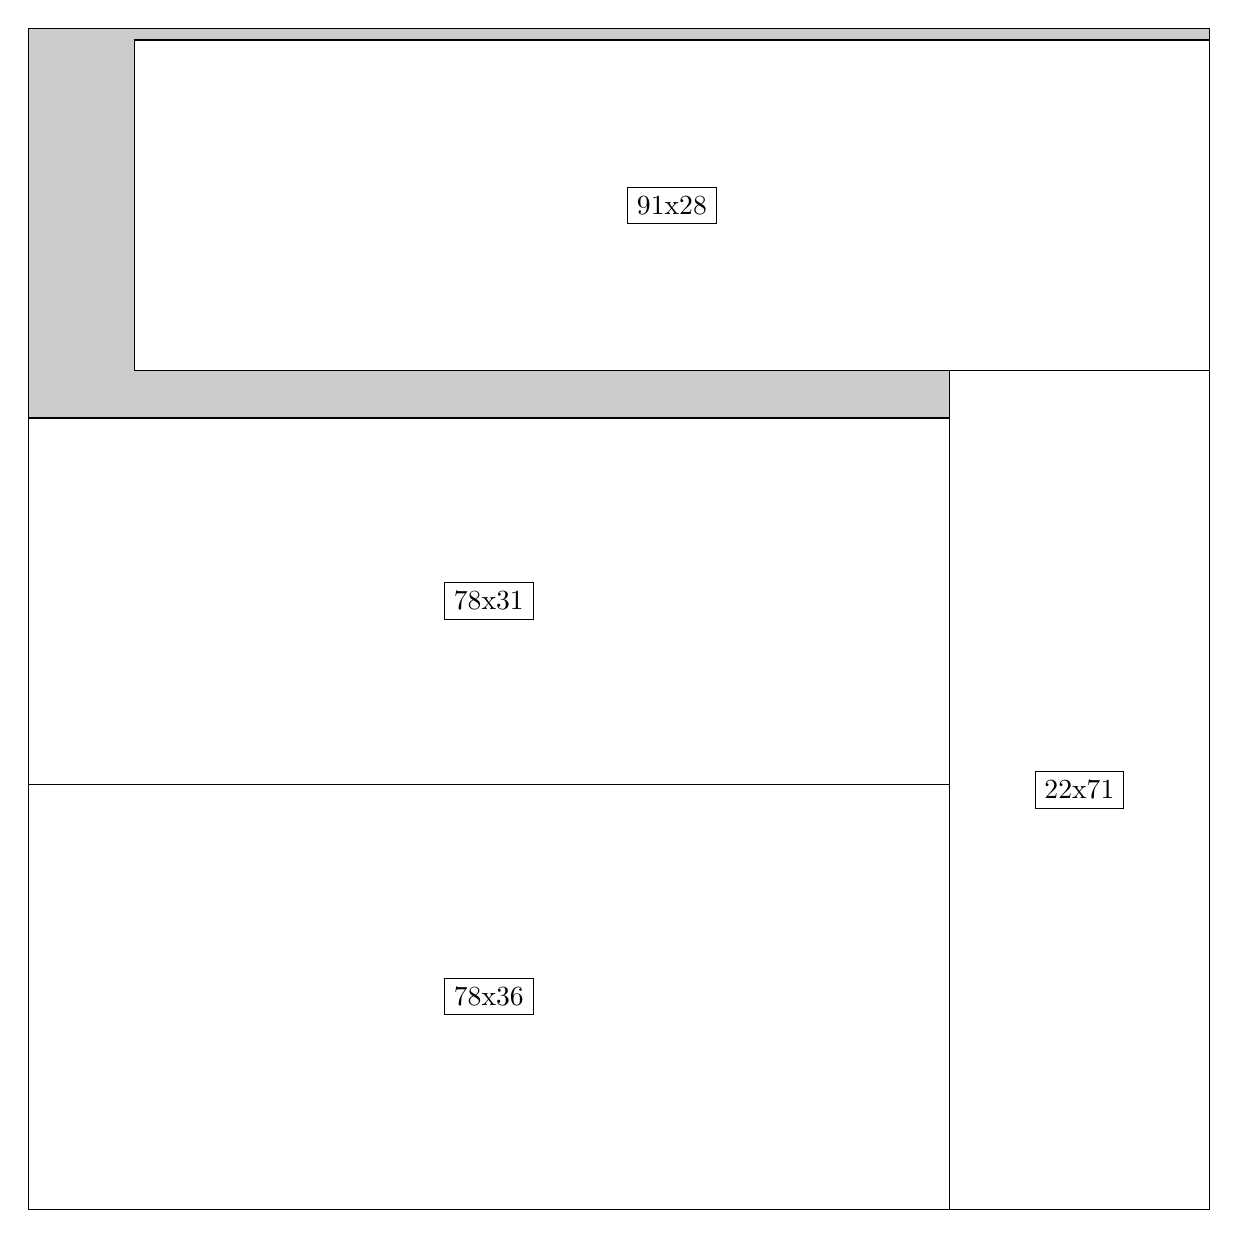
\begin{tikzpicture}[shorten >=1pt,scale=1.0,every node/.style={scale=1.0},->]
\tikzstyle{vertex}=[circle,fill=black!25,minimum size=14pt,inner sep=0pt]
\filldraw[fill=gray!40!white, draw=black] (0,0) rectangle (15.0,15.0);
\foreach \name/\x/\y/\w/\h in {78x36/0.0/0.0/11.7/5.3999999999999995,91x28/1.3499999999999999/10.65/13.65/4.2,78x31/0.0/5.3999999999999995/11.7/4.6499999999999995,22x71/11.7/0.0/3.3/10.65}
\filldraw[fill=white!40!white, draw=black] (\x,\y) rectangle node[draw] (\name) {\name} ++(\w,\h);
\end{tikzpicture}


w =78 , h =36 , x =0 , y =0 , v =2808
\par
w =91 , h =28 , x =9 , y =71 , v =2548
\par
w =78 , h =31 , x =0 , y =36 , v =2418
\par
w =22 , h =71 , x =78 , y =0 , v =1562
\par
\newpage


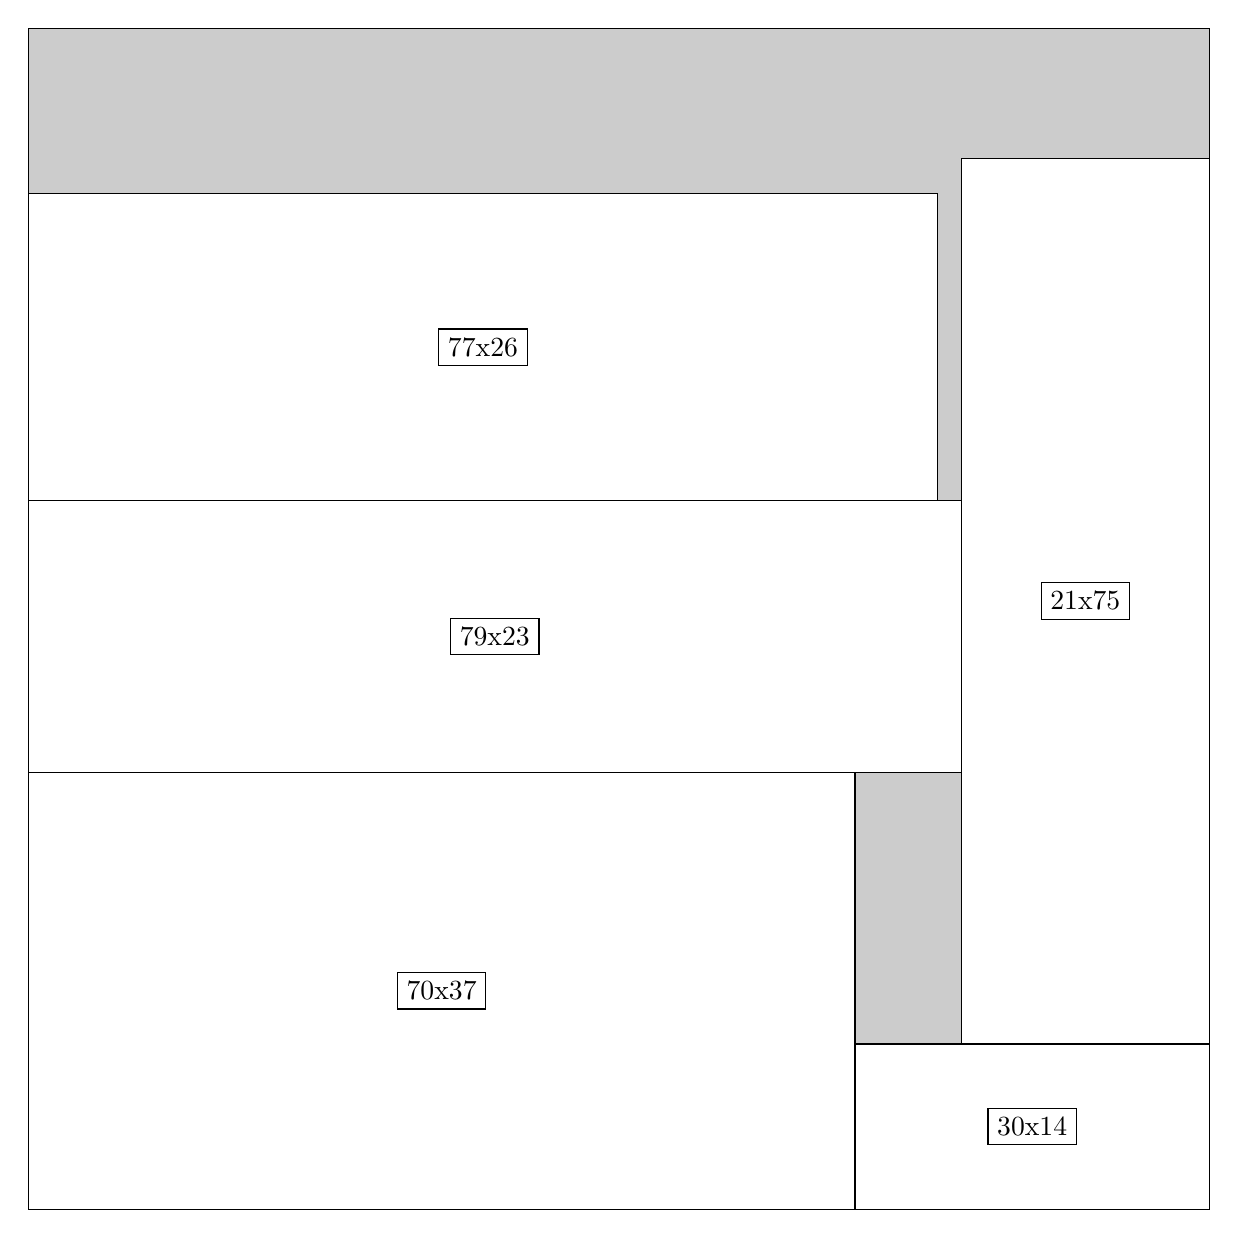
\begin{tikzpicture}[shorten >=1pt,scale=1.0,every node/.style={scale=1.0},->]
\tikzstyle{vertex}=[circle,fill=black!25,minimum size=14pt,inner sep=0pt]
\filldraw[fill=gray!40!white, draw=black] (0,0) rectangle (15.0,15.0);
\foreach \name/\x/\y/\w/\h in {70x37/0.0/0.0/10.5/5.55,77x26/0.0/9.0/11.549999999999999/3.9,79x23/0.0/5.55/11.85/3.4499999999999997,21x75/11.85/2.1/3.15/11.25,30x14/10.5/0.0/4.5/2.1}
\filldraw[fill=white!40!white, draw=black] (\x,\y) rectangle node[draw] (\name) {\name} ++(\w,\h);
\end{tikzpicture}


w =70 , h =37 , x =0 , y =0 , v =2590
\par
w =77 , h =26 , x =0 , y =60 , v =2002
\par
w =79 , h =23 , x =0 , y =37 , v =1817
\par
w =21 , h =75 , x =79 , y =14 , v =1575
\par
w =30 , h =14 , x =70 , y =0 , v =420
\par
\newpage


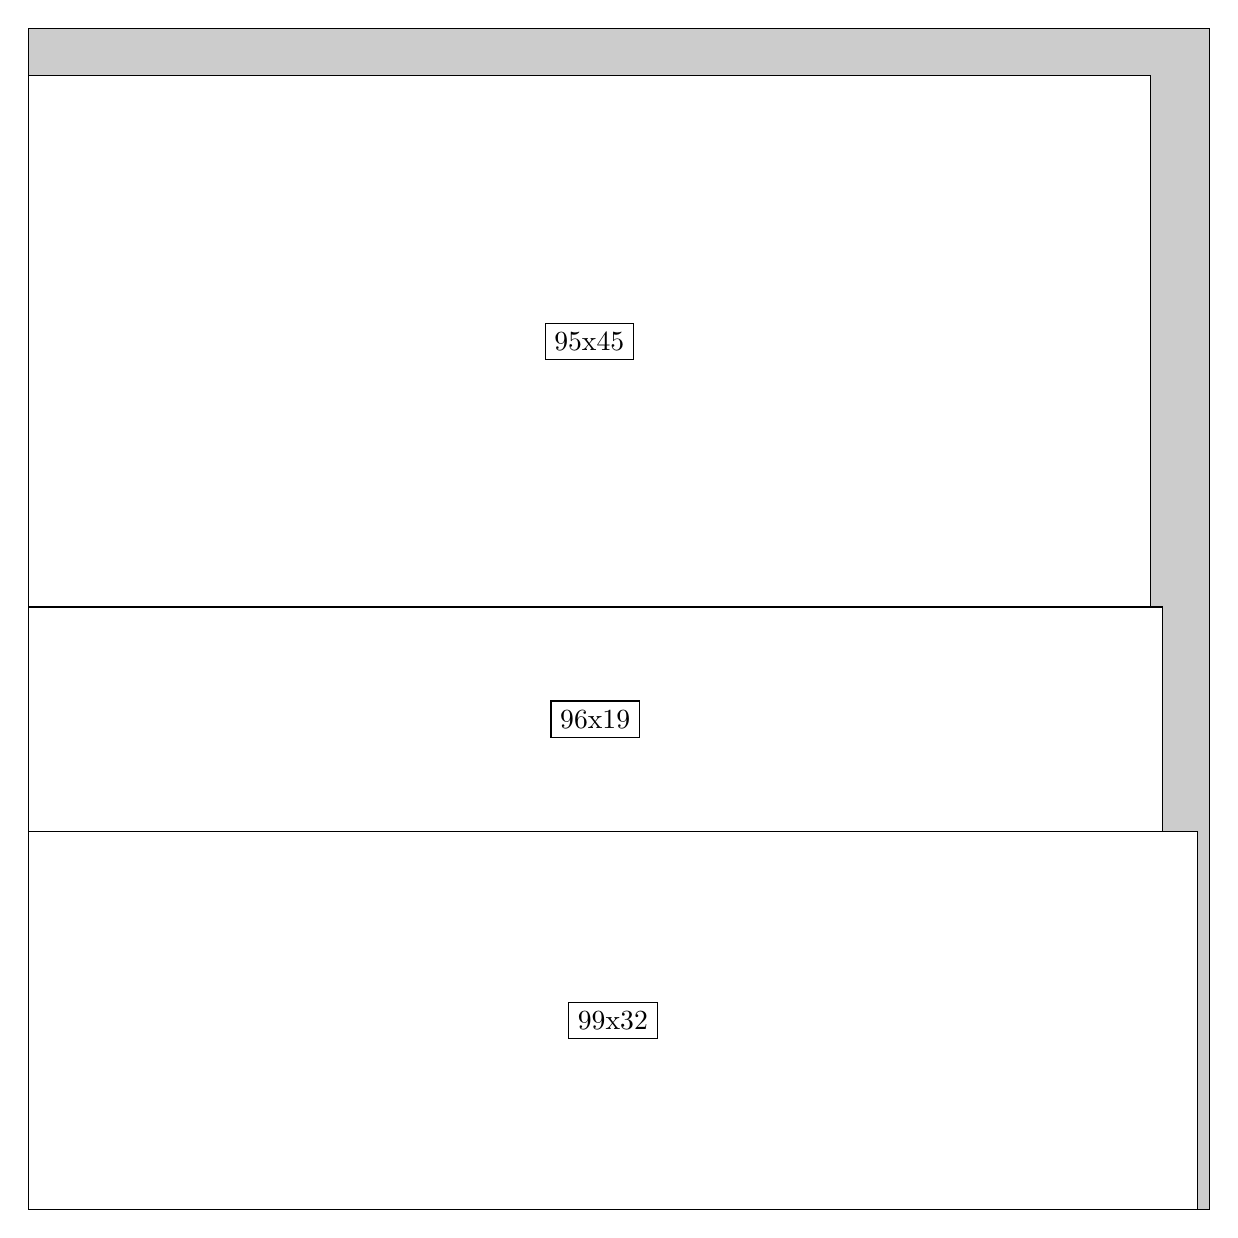
\begin{tikzpicture}[shorten >=1pt,scale=1.0,every node/.style={scale=1.0},->]
\tikzstyle{vertex}=[circle,fill=black!25,minimum size=14pt,inner sep=0pt]
\filldraw[fill=gray!40!white, draw=black] (0,0) rectangle (15.0,15.0);
\foreach \name/\x/\y/\w/\h in {95x45/0.0/7.6499999999999995/14.25/6.75,99x32/0.0/0.0/14.85/4.8,96x19/0.0/4.8/14.399999999999999/2.85}
\filldraw[fill=white!40!white, draw=black] (\x,\y) rectangle node[draw] (\name) {\name} ++(\w,\h);
\end{tikzpicture}


w =95 , h =45 , x =0 , y =51 , v =4275
\par
w =99 , h =32 , x =0 , y =0 , v =3168
\par
w =96 , h =19 , x =0 , y =32 , v =1824
\par
\newpage


\end{document}